\chapter{Resultados}

En esta sección se va a mostrar los resultados obtenidos con el modelo propuesto. Se va a usar el conjunto de datos reducido ya que es necesario ejecutar reiteradas veces el modelo. En la versión
propuesta del modelo solo tenemos dos hiperparámetros:
\begin{itemize}
  \item Ratio de aprendizaje
  \item Tamaño del \textit{embedding}
\end{itemize}

En la figura \ref{embedding_size} se muestra la evolución de la pérdida del modelo durante 100 épocas para varios tamaños de \textit{embedding}. Como se aprecia en la figura, no hay diferencias significativas
en la velocidad de aprendizaje. Se puede apreciar que el modelo mejora rápidamente en las primeras épocas. No obstante, en las siguientes el ritmo de aprendizaje es mucho más moderado y casi imperceptible
en la gráfica.

En las tablas \ref{w50} y \ref{w75} y \ref{w100} se puede ver en la primera columna algunos tropos del vocabulario. En las otras columnas se muestran, por orden, los dos tropos más similares
al de la primera columna. Entre paréntesis se muestra la similitud coseno de sus respectivos \textit{embeddings}. En las tres tablas se muestran los mismos tropos en la misma columna. Como se puede observar,
hay algunas repeticiones como el tropo \textit{InUniverse} para el tropo \textit{ActorAllusion}. Esto parece indicar que independientemente del tamaño del \textit{embedding}, el modelo aprende más o menos las mismas
relaciones entre los distintos tropos.

\begin{figure}\label{embedding_size}[H]
  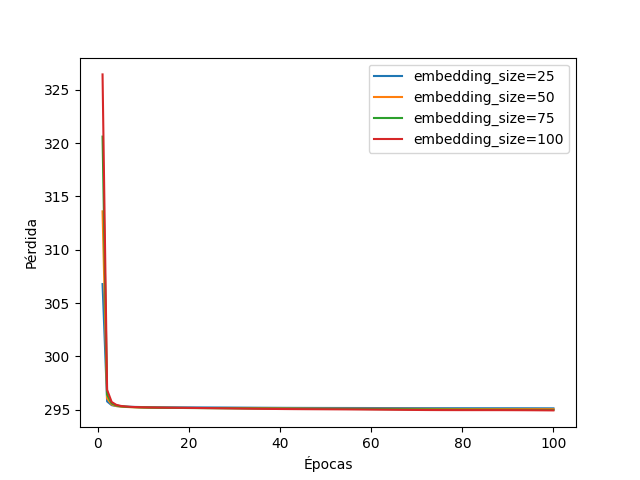
\includegraphics[width=12cm]{perdida.png}
  \centering
  \caption{La pérdida es medida usando la función \ref{perdida_1}}
\end{figure}

\begin{center}
  \begin{table}
  \resizebox{\textwidth}{!}{%
  \begin{tabular}{|c|c|c|}
  \hline
  Tropo & 0 & 1\\
  \hline
  AbusiveParents & FilmsDiscussedByMoviebob(0.59) & ForegoneConclusion(0.59)\\
  \hline
  ActionGirl & ChekhovsGunman(0.65) & DeadpanSnarker(0.54)\\
  \hline
  ActorAllusion & InUniverse(0.68) & MyGodWhatHaveIDone(0.65)\\
  \hline
  \end{tabular}}
  \caption{Tropos similares usando \textit{embeddings} de tamaño 50}
  \label{w50}
  \end{table}
\end{center}


\begin{center}
  \begin{table}
  \resizebox{\textwidth}{!}{%
  \begin{tabular}{|c|c|c|}
  \hline
  Tropo & 0 & 1\\
  \hline
  AbusiveParents & CreatorCameo(0.53) & JustForFun(0.49)\\
  \hline
  ActionGirl & TearJerker(0.6) & TroubledProduction(0.54)\\
  \hline
  ActorAllusion & ActionGirl(0.42) & TearJerker(0.41)\\
  \hline
  \end{tabular}}
  \caption{Tropos similares usando \textit{embeddings} de tamaño 75}
  \label{w75}
  \end{table}
\end{center}


\begin{center}
\begin{table}
  \resizebox{\textwidth}{!}{%
  \begin{tabular}{|c|c|c|}
  \hline
  Tropo & 0 & 1\\
  \hline
  AbusiveParents & Tagline(0.45) & FilmsDiscussedByMoviebob(0.41)\\
  \hline
  ActionGirl & TroubledProduction(0.4) & GrandUnifiedTimeline(0.35)\\
  \hline
  ActorAllusion & NiceJobBreakingItHero(0.42) & InUniverse(0.37)\\
  \hline
  \end{tabular}}
  \caption{Tropos similares usando \textit{embeddings} de tamaño 100}
  \label{w100}
\end{table}
\end{center}

En la figura \ref{tsne_full} se puede ver la representación del resultado del modelo t-SNE (usado para representar datos con alta dimensionalidad en dos o tres dimensiones y detectar agrupaciones en los datos)
para los \textit{embeddings} de tamaño 100 y ratio de aprendizaje 0.001.
En el repositorio del trabajo se encontrar la imagen a tamaño completo. En la figura \ref{tsne} se aprecia una versión amplificada de la gráfica anterior donde
se pueden apreciar algunos de los tropos.

\begin{figure}\label{tsne_full}
  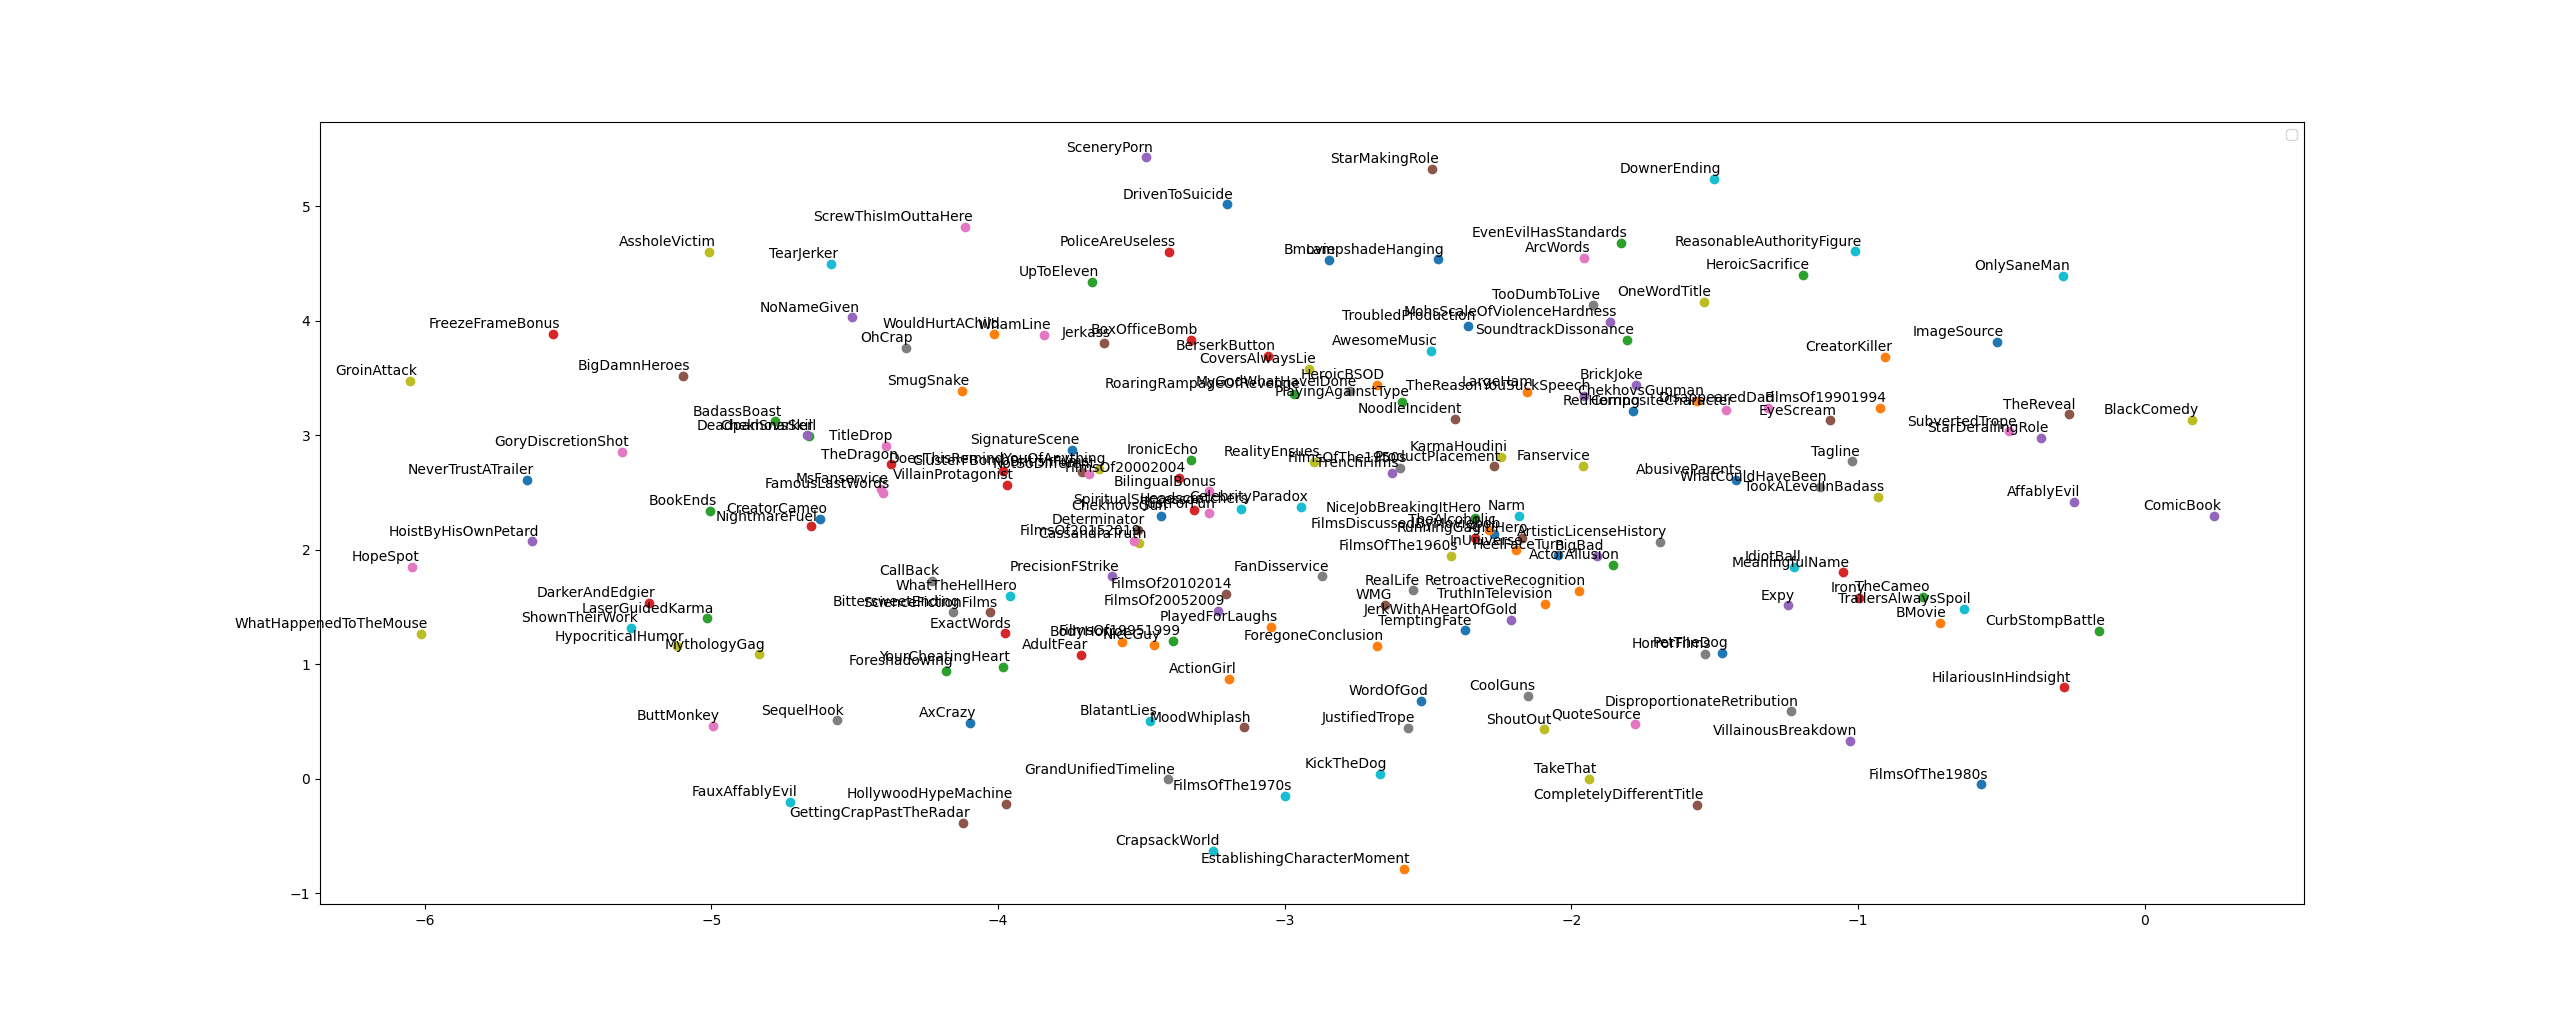
\includegraphics[width=12cm]{tsne_full.png}
  \centering
  \caption{Resultado de t-SNE para el conjunto de datos reducido}
\end{figure}

\begin{figure}\label{tsne}
  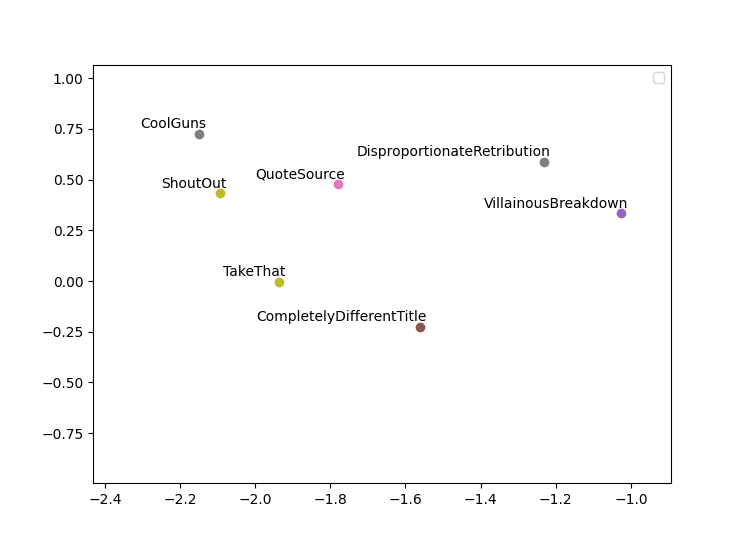
\includegraphics[width=12cm]{tsne.png}
  \centering
  \caption{Ampliación del resultado de t-SNE para el conjunto de datos reducido}
\end{figure}

Se puede apreciar que después de 2500 iteraciones del modelo, la nube de puntos sigue bastante dispersa. Esto indica que el algoritmo no ha sido capaz de encontrar
agrupaciones significativas de tropos. Por un lado es razonable que no se hayan encontrado agrupaciones significantes ya que en el conjunto de datos no se ha incluido
información significante para que esto ocurra (como por ejemplo se hace en \cite{kazama2018neural} con el país de la receta). Sin embargo, se esperaban detectar algunas
agrupaciones: como por ejemplo, haber encontrado `tipos' o `estilos' de tropos.

Una vez se han conseguido los \textit{embeddings} también se pueden sumar y restar entre ellos. Por ejemplo:
\begin{equation}
  \text{AntiHero} - \text{ArcWords} = \text{ForegoneConclusion}
\end{equation}
Consultando el significado de estos tropos:
\begin{itemize}
  \item \textit{AntiHero}: representa a los antihéroes.
  \item \textit{ArcWords}: representa alguna frase simbólica que aparece reiteradas veces a lo largo de un arco argumental.
  \item \textit{ForegoneConclusion}: representa cuando el autor anuncia el final al principio de la obra pero no explica cómo se llega hasta ahí.
\end{itemize}

\begin{figure}\label{ampliacion_meta}
  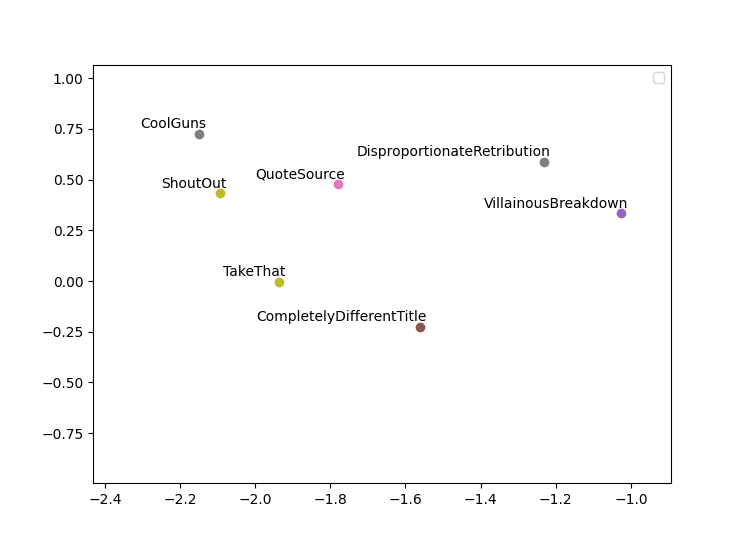
\includegraphics[width=12cm]{tsne.png}
  \centering
  \caption{Ampliación del resultado de t-SNE}
\end{figure}

En la ampliación \ref{ampliacion_meta} se pueden observar que varios tropos (\textit{Bmovie}, \textit{TrailersAlwaysSpoil} y \textit{MeaningfulName}) que son considerados \textit{meta}. Estos tropos no son narrativos,
es decir, no describen la trama de la película, sino características de ella. Por ejemplo, \textit{B-Movie}, un tropo usado para describir aquellas películas con un bajo presupuesto.

\begin{figure}\label{ampliacion_fecha}
  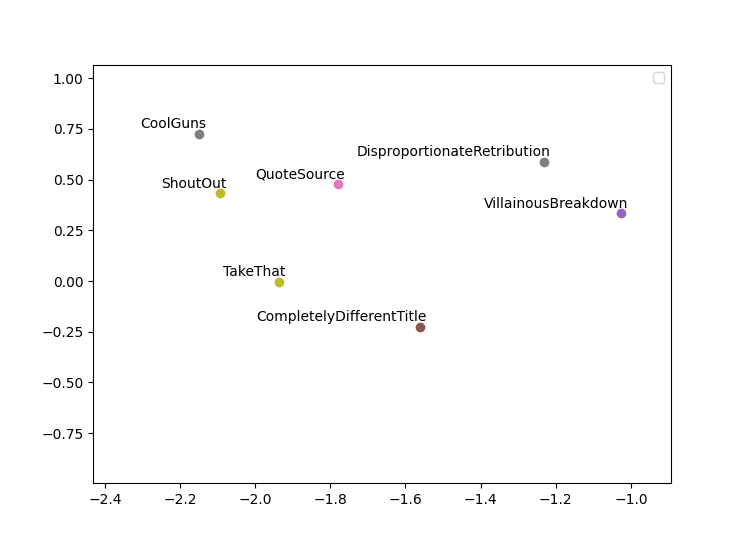
\includegraphics[width=12cm]{tsne.png}
  \centering
  \caption{Ampliación del resultado de t-SNE}
\end{figure}

En la ampliacion \ref{ampliacion_fecha} se puede ver el meta tropo \textit{FilmsOfThe1970s}, usado para representar películas de la década de los 70. A su alrededor se encuentran
\textit{KickTheDog} y \textit{GranUnifiedTimeline}, tropos que se hicieron populares en esa década.

Como se puede ver, se ha obtenido información adicional de los tropos en algunos casos, mientras que se no se han conseguido los resultados esperados en otros.
Esto junto con el hecho de no haber encontrado agrupaciones entre tropos, indica que no se ha sido capaz
de resolver el problema propuesto de una forma satisfactoria. Sin embargo, sí se ha conseguido extender el modelo \textit{Word2Vec} a \textit{Any2Vec}. Esto significa
que futuros investigadores o personas interesadas pueden continuar el trabajo con los tropos o incluso aplicar el modelo a otro tipo de datos, como recetas \cite{kazama2018neural}.